\subsection{Propositional Resolution Calculus}
\label{sec:resolution}

In this section, we will define the propositional resolution calculus.
Resolution is one of the most well known automated deduction techniques and goes back to Robinson \cite{Robinson1965}.
While it is a pretty simple calculus with just one inference rule, proofs in that calculus tend to become large.
This property and its popularity make it a good target for proof compression.

Propositional resolution can be seen as a simplification of first-order logic resolution to propositional logic.
For basics about propositional logic and its prominent decision problem SAT, we refer the reader to \cite{Biere2009}.
For an extensive discussion of propositional and first-order logic resolution, we refer the reader to \cite{Leitsch1997}.

\begin{definition}[Literal and Clause]

A \emph{literal} is a propositional variable or the negation of a propositional variable. 
The \emph{complement} of a literal $\ell$ is denoted $\dual{\ell}$ (i.e. for any propositional variable $p$,
$\dual{p} = \neg p$ and $\dual{\neg p} = p$). 
A \emph{clause} is a set of literals. 
$\bot$ denotes the \emph{empty clause}.

\end{definition}

A clause represents the propositional logic formula that is the disjunction of its literals.
A set of clauses represents the formula that is the conjunction of its clauses.
The propositional resolution calculus operates on propositional formulas in conjunctive normal form, which are formulas that are represented by a set of clauses.

\begin{definition}[Resolvent]

Let $C_1$ and $C_2$ be two different clauses and $\ell$ be a literal, such that $\ell \in C_1$ and $\dual{\ell} \in C_2$.
The clause $C_1 \setminus \{\ell\} \cup C_2 \setminus \{\dual{\ell}\}$ is called the \emph{resolvent} of $C_1$ and $C_2$ with \emph{pivot} $\ell$.

\end{definition}

The condition of $C_1$ and $C_2$ being different technically is not necessary.
However if it is possible to resolve a clause with itself, then the clause contains both the positive and negative version of a variable and is therefore tautological (i.e. trivially satisfiable).
Since the resolution calculus is refutational, i.e. it seeks to show unsatisfiability, such clauses are of no use and therefore we ignore them.
In case it is possible to produce a resolvent of two clauses w.r.t. two different literals, no matter which literal is chosen, the resulting resolvent will be tautological.
Therefore the choice of literal to resolve on is not an interesting question to investigate and we will drop the reference to the literal when speaking about resolvents.
In terms of proof calculi, axioms of the propositional resolution calculus are clauses and the single rule of the calculus is to derive a resolvent from previously derived clauses or axioms.
This work studies the syntactic and semantic structure of derivations in this calculus, which are formally defined in the following.

\begin{definition}[Resolution Derivation and Refutation]

Let $F = \{C_1, \ldots, C_n\}$ be a set of clauses.
The notion of a \emph{resolution derivation} for $F$ is defined inductively.
\begin{itemize}
	\item $\langle C_1, \ldots, C_n\rangle$ is a resolution derivation for $F$.
	\item If $\langle C_1, \ldots, C_m\rangle$ is a resolution derivation for $F$ then $\langle C_1, \ldots, C_{m+1} \rangle$ is a resolution derivation for $F$ if $C_{m+1}$ is a resolvent of $C_i$ and $C_j$ with $1 \leq i,j \leq m$.
\end{itemize}
A \emph{resolution refutation} is a resolution derivation containing the empty clause.

\end{definition}

The correctness of the resolution calculus can be formulated as the statement, that a propositional logic formula, represented as a set of clauses, imply all clauses of all resolution derivations of it. 
Since the empty clause is unsatisfiable and a formula with a resolution derivation that is a refutation is unsatisfiable.
Therefore a resolution refutation of $F$ is a witness to the validity of $\neg F$.
For an unsatisfiable formula, there can be many different resolution refutations.
The aim of proof compression is to find short refutations among all possible ones.

We prefer a different view on refutations, which is more suited for the purpose of proof manipulation.
In the following definition, we present proofs as labeled graphs.

\begin{definition}[Proof] 
\label{def:proof}
A \emph{proof} $\varphi$ is a labeled directed acyclic graph $\langle V,E,\n,\mathcal{L} \rangle$, such that $\n$ has no incoming edges.
The labeling function $\mathcal{L}$ maps nodes to clauses.
The designated node $\n \in V$ is the root of the graph, i.e. it is a node without children and every node of the graph is a recursive ancestor of the node.
Furthermore, a proof has to fulfill one of the following properties:

\begin{enumerate}
	\item $V = \{\n\}, E = \emptyset$
	\item \label{enum:resCase} 
		There are proofs $\varphi_L = \langle V_L, E_L, \n_L,\mathcal{L}_1 \rangle$ and $\varphi_R = \langle V_R, E_R, \n_R, \mathcal{L}_2 \rangle$ such that 
		$\n \notin (V_L \cup V_R)$, $\mathcal{L}_1(x) = \mathcal{L}_2(x)$ for every $x \in (V_L \cap V_R)$,
		$\mathcal{L}(\n)$ is the resolvent of $\mathcal{L}(\n_L)$ and $\mathcal{L}(\n_R)$ w.r.t. some literal $\ell$,
		for $x \in V_L: \mathcal{L}(x) = \mathcal{L}_1(x)$ and for $x \in V_R: \mathcal{L}(x) = \mathcal{L}_2(x)$,
		$V = (V_L \cup V_R) \cup \{\n \}$, $E = E_L \cup E_R \cup \{(\n_L,\n) , (\n_R,\n) \}$.
\end{enumerate}

The node $\n$ is called the \emph{root} of $\varphi$ and $\mathcal{L}(\n)$ its \emph{conclusion}.
In case \ref{enum:resCase}, $\varphi_L$ and $\varphi_R$ are \emph{premises} of $\varphi$ and $\varphi$ is a \emph{child} of $\varphi_L$ and $\varphi_R$.
A proof $\psi$ is a subproof of a proof $\varphi$, if they are related in the transitive closure of the premise relation.
A subproof $\psi$ of $\varphi$ which has no premises is an \emph{axiom} of $\varphi$.
$\Vertices{\varphi}$ and $\Axioms{\varphi}$ denote, respectively, the set of nodes and axioms of $\varphi$. 
$\Premises{\n}{\varphi}$ denotes the premises and $\Children{\n}{\varphi}$ the children of the subproof with root $\n$ in a proof $\varphi$. 
When a proof is represented graphically, the root is drawn at the bottom and the axioms at the top. 
The \emph{length} of a proof $\varphi$ is the number of nodes in $\Vertices{\varphi}$ and is denoted by $\plength{\varphi}$.
\end{definition}

Other measures of proofs that are not discussed in this work are height, width and size of the unsat core.

\noindent
Note that since the labeling of premises must agree on common nodes and edges, the definition of the labeling $\mathcal{L}$ is unambiguous.
Also note that in case \ref{enum:resCase} of Definition \ref{def:proof} $V_L$ and $V_R$ are not required to be disjoint. 
Therefore the underlying structure of a proof is really a directed acyclic graph and not simply a tree. 
Modern SAT- and SMT-solvers, using techniques of conflict driven clause learning, produce proofs with a  DAG structure \cite{Bouton2009,Biere2009}.
The reuse of proof nodes plays a central role in proof compression \cite{Fontaine2011}.

\begin{example}

Consider the propositional logic formula $\Phi$ in conjunctive normal form.
$$\Phi := (x_1 \vee \neg x_2 \vee \neg x_3) \wedge (x_1 \vee x_2) \wedge (x_1 \vee x_3) \wedge (\neg x_1)$$
In clause notation, this formula is written as $\langle \{x_1, \neg x_2, \neg x_3\}, \{x_1, x_2\}, \{x_1, x_3\}, \{\neg x_1\} \rangle$.
By resolving the clauses $\{x_1, \neg x_2, \neg x_3\}$ and $\{x_1, x_2\}$, we obtain the clause $\{x_1,\neg x_3\}$, which we can resolve with $\{x_1, x_3\}$ to obtain $\{x_1\}$.
Finally, we obtain the empty clause $\bot$ by resolving $\{x_1\}$ with $\{\neg x_1\}$.
The resulting proof is shown graphically in Figure \ref{fig:resolutionexample}.
Figure \ref{fig:resolutionexample2} shows a proof of the same formula, which is longer than the one proof we presented.

\begin{figure}[!ht]

\centering
\begin{tikzpicture}[node distance=1.5cm]

	\rootnode;
	
	\withchildren{root} {nx1}{$\{\neg x_1\}$} {x1}{$\{x_1\}$};
	\withchildren{x1}{n3}{$\{x_1,\neg x_3\}$} {n4} {$\{x_1, x_3\}$};
	\withchildren{n3}{n1}{$\{x_1,\neg x_2,\neg x_3\}$} {n4} {$\{x_1, x_2\}$};

\end{tikzpicture}

\caption{Proof of $\Phi$'s unsatisfiability}
\label{fig:resolutionexample}
\end{figure}

\begin{figure}[!ht]

\centering
\begin{tikzpicture}[node distance=1.5cm]

	\rootnode;
	
	\proofnode[above right of=root]{ghost}{};
	\proofnode[above left of=root]{n6}{$\{x_3\}$};
	\proofnode[above right of=ghost]{n8}{$\{\neg x_3\}$};
	\drawchildren{root}{n6}{n8};
	\withchildren{n6}{n3}{$\{\neg x_2,x_3\}$} {n5} {$\{x_2\}$};
	\withchildren{n3}{n1}{$\{x_1,\neg x_2,\neg x_3\}$} {n2} {$\{\neg x_1\}$};
	\proofnode[above right of=n5]{n4} {$\{x_1,x_2\}$};
	\drawchildren{n5}{n2}{n4};
	
	\proofnode[above right of=n8]{n7} {$\{x_1,\neg x_3\}$};
	\drawchildren{n8}{n7}{n2};
	
\end{tikzpicture}

\caption{Another Proof of $\Phi$'s unsatisfiability}
\label{fig:resolutionexample2}
\end{figure}

\end{example}